\documentclass[10pt,a4paper]{article}
\usepackage[utf8]{inputenc}
\usepackage[italian]{babel}
\usepackage[a4paper]{geometry}
\usepackage{amsmath}
\usepackage{amsthm}
\usepackage{dsfont}
\usepackage{xfrac}
\usepackage{amsfonts}
\usepackage{amssymb}
\usepackage{graphicx}
\usepackage{braket}
\usepackage{mathtools}
\usepackage{booktabs}
\usepackage{hyperref}
\usepackage{enumerate}
\DeclarePairedDelimiterX{\norm}[1]{\lVert}{\rVert}{#1}
\theoremstyle{plain}
\newtheorem{definizione}{Definizione}
\theoremstyle{definition}
\newtheorem{teorema}{Teorema}
\newtheorem{dimostrazione}{Dimostrazione}
\newtheorem{corollario}{Corollario}
\newtheorem{osservazione}{Osservazione}
\newtheorem{proposizione}{Proposizione}
\newtheorem{esempio}{Esempio}
%%%%%%%INSERIAMO QUI I NUOVI COMANDI %%%%%%%%%%%%%%%%%%%%%%%%%%%%%%%%%%%%%%%%%%%%
\DeclarePairedDelimiterX{\abla}[1]{abla}{abla}{#1}

%%%%%%%QUI VANNO INSERITI IL TITOLO E GLI AUTORI%%%%%%%%%%%%%%%%%%%%%%%%%%%%
\author{Andrea Zanin}
\title{Appunti Matematica Fisica - Andata e Ritorno}
\date{6 June 2017}
\begin{document}
	\maketitle
	\section{Vettori}
	Alcune operazioni tra vettori:
	\[P_1=(x_1,y_1) \qquad P_2=(x_2,y_2)\qquad r \in \mathbb{R}\]
	\begin{definizione} Somma tra vettori
		\label{vec:sum}
		\[P_1 + P_2 = (x_1+x_2, y_1+y_2)\]
	\end{definizione}
	\begin{definizione} Moltiplicazione per un numero
		\label{vec:nprod}
		\[r\cdot P=(r\cdot x_1, r\cdot y_2)\]
	\end{definizione}
	\subsection{Prodotto scalare}
	\begin{definizione} Prodotto scalare
		\label{vec:sprod}
		\[P_1 \cdot P_2 := x_1 \cdot x_2 + y_1 \cdot y_2\]
	\end{definizione}
	\begin{itemize}
		\item Commutatività $P_1 \cdot P_2 = P_2 \cdot P_1$
		\item Linearità $(P_1 + P_2)\cdot P_3 = P_1 \cdot P_3 + P_2 \cdot P_3$
		\item omogeneità $(r\cdot P_1)P_2 = r(P_1 \cdot P_2)$
		\item norma $\norm{P}=\sqrt{x^2 + y^2}$
	\end{itemize}
	\begin{teorema} $P_1 \cdot P_2 = \norm{P_1} \cdot \norm{P_2} \cdot \cos{\theta}$
	
	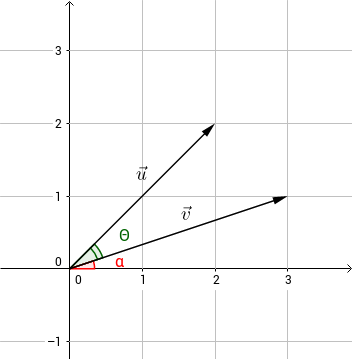
\includegraphics[scale=0.5]{graph.png}
	
	\begin{align*}
		P_1\cdot P_2 &= x_1 x_2 + y_1 y_2 \\
		&=\norm{P_1}\cdot \cos{(\alpha)} \cdot \norm{P_2} \cdot \cos{(\alpha + \theta)} + \norm{P_1}\cdot \sin{(\alpha)} \cdot  \norm{P_2} \cdot \sin{(\alpha + \theta)} \\
		&=\norm{P_1}\cdot \norm{P_2}(\cos{(\alpha)} \cdot \cos{(\alpha + \theta)} + \sin{(\alpha)} \cdot \sin{(\alpha + \theta)}) \\
		& = \norm{P_1} \cdot \norm{P_2} \cdot \cos{(\theta)} \\
		&&\Box
	\end{align*}	
	\end{teorema}
	
	\begin{osservazione} 
		Se il prodotto scalare di 2 vettori diversi da 0 è nullo i 2 vettori devono essere perpendicolari
	\end{osservazione}
	
	\begin{definizione} Il "ruotato" di un vettore è il vettore stesso ruotato di 90°
		\[P=(a,b)\]
		\[R(P)=(-b,a)\]
	\end{definizione}
	\begin{osservazione}
		$P_1 \parallel P_2 \Leftrightarrow P_1 \cdot (R(P_2))=0$
	\end{osservazione}
	\section{Matrici}
	\begin{definizione}
		Una matrice è una tabella di numeri
		\[\begin{pmatrix}
			a & b \\
			c & d
		\end{pmatrix}\]
	\end{definizione}
	\begin{osservazione}
		Possiamo interpretare la matrice come 2 vettori in riga o in colonna:
		\[
		a=(a_1,a_2) \qquad b=(b_1,b_2)
		\]
		\[
		M=(a|b)=
		\begin{pmatrix}
		a_1 & b_1 \\
		a_2 & b_2
		\end{pmatrix}
		\]
		\[
		M=
		\left(
		\begin{array}{cc}
		a\\ \midrule
		b
		\end{array}
		\right)
		\]
	\end{osservazione}
	\begin{definizione}
		Prodotto tra una matrice e un vettore
		\[
		M(P)= \left(
		\begin{array}{cc}
		a\\ \midrule
		b
		\end{array}
		\right)
		P
		:=
		\left(
		\begin{array}{cc}
		a \cdot P\\ \midrule
		b \cdot P
		\end{array}
		\right)
		\]
	\end{definizione}
	\begin{osservazione}
		Possiamo interpretare una matrice come una funzione che associa a punti nello spazio altri punti nello spazio
	\end{osservazione}
	\begin{dimostrazione}$M(P)=x\vec{u}  + y \vec{v}$\\
		Ipotesi
		\[
		M=(u|v)=
		\begin{pmatrix}
		u_1 & v_1 \\
		u_2 & v_2
		\end{pmatrix}
		\qquad 
		P=\begin{pmatrix}
			x \\
			y
		\end{pmatrix}
		\]
		Tesi
		\[
		M(P)=x\vec{u}  + y \vec{v}
		\]
		Dimostrazione
		\begin{align*}
			M(P)&=(u|v)P \\
			&=\begin{pmatrix}
			u_1 & v_1 \\
			u_2 & v_2
			\end{pmatrix}
			\begin{pmatrix}
			x \\
			y
			\end{pmatrix}
			\\
			&=\begin{pmatrix}
			u_1x + v_1y \\
			u_2x + v_2y
			\end{pmatrix}
			\\
			&=\begin{pmatrix}
			u_1x \\
			u_2x
			\end{pmatrix}
			+
			\begin{pmatrix}
			v_1y \\
			v_2y
			\end{pmatrix}
			\\
			&=x\begin{pmatrix}
			u_1 \\
			u_2
			\end{pmatrix}
			+
			y\begin{pmatrix}
			v_1 \\
			v_2
			\end{pmatrix}
			\\
			&=x\vec{u}  + y \vec{v}
			\\
			&&\Box
		\end{align*}
	\end{dimostrazione}
	\begin{corollario}Dalla dimostrazione precedente deduciamo che
		\[
		M\begin{pmatrix}
		1 \\
		0
		\end{pmatrix}
		= \vec{u}
		\]
		\[
		M\begin{pmatrix}
		0 \\
		1
		\end{pmatrix}
		= \vec{v}
		\]
	\end{corollario}
	\begin{osservazione}La matrice è un operatore lineare
		\[
		M(\alpha P_1 + \beta P_2)= \alpha M(P_1) + \beta M(P_2)
		\]
	Possiamo comprende intuitivamente questa affermazione osservando con una rappresentazione grafica della trasformazione che la matrice rappresenta\\
	
	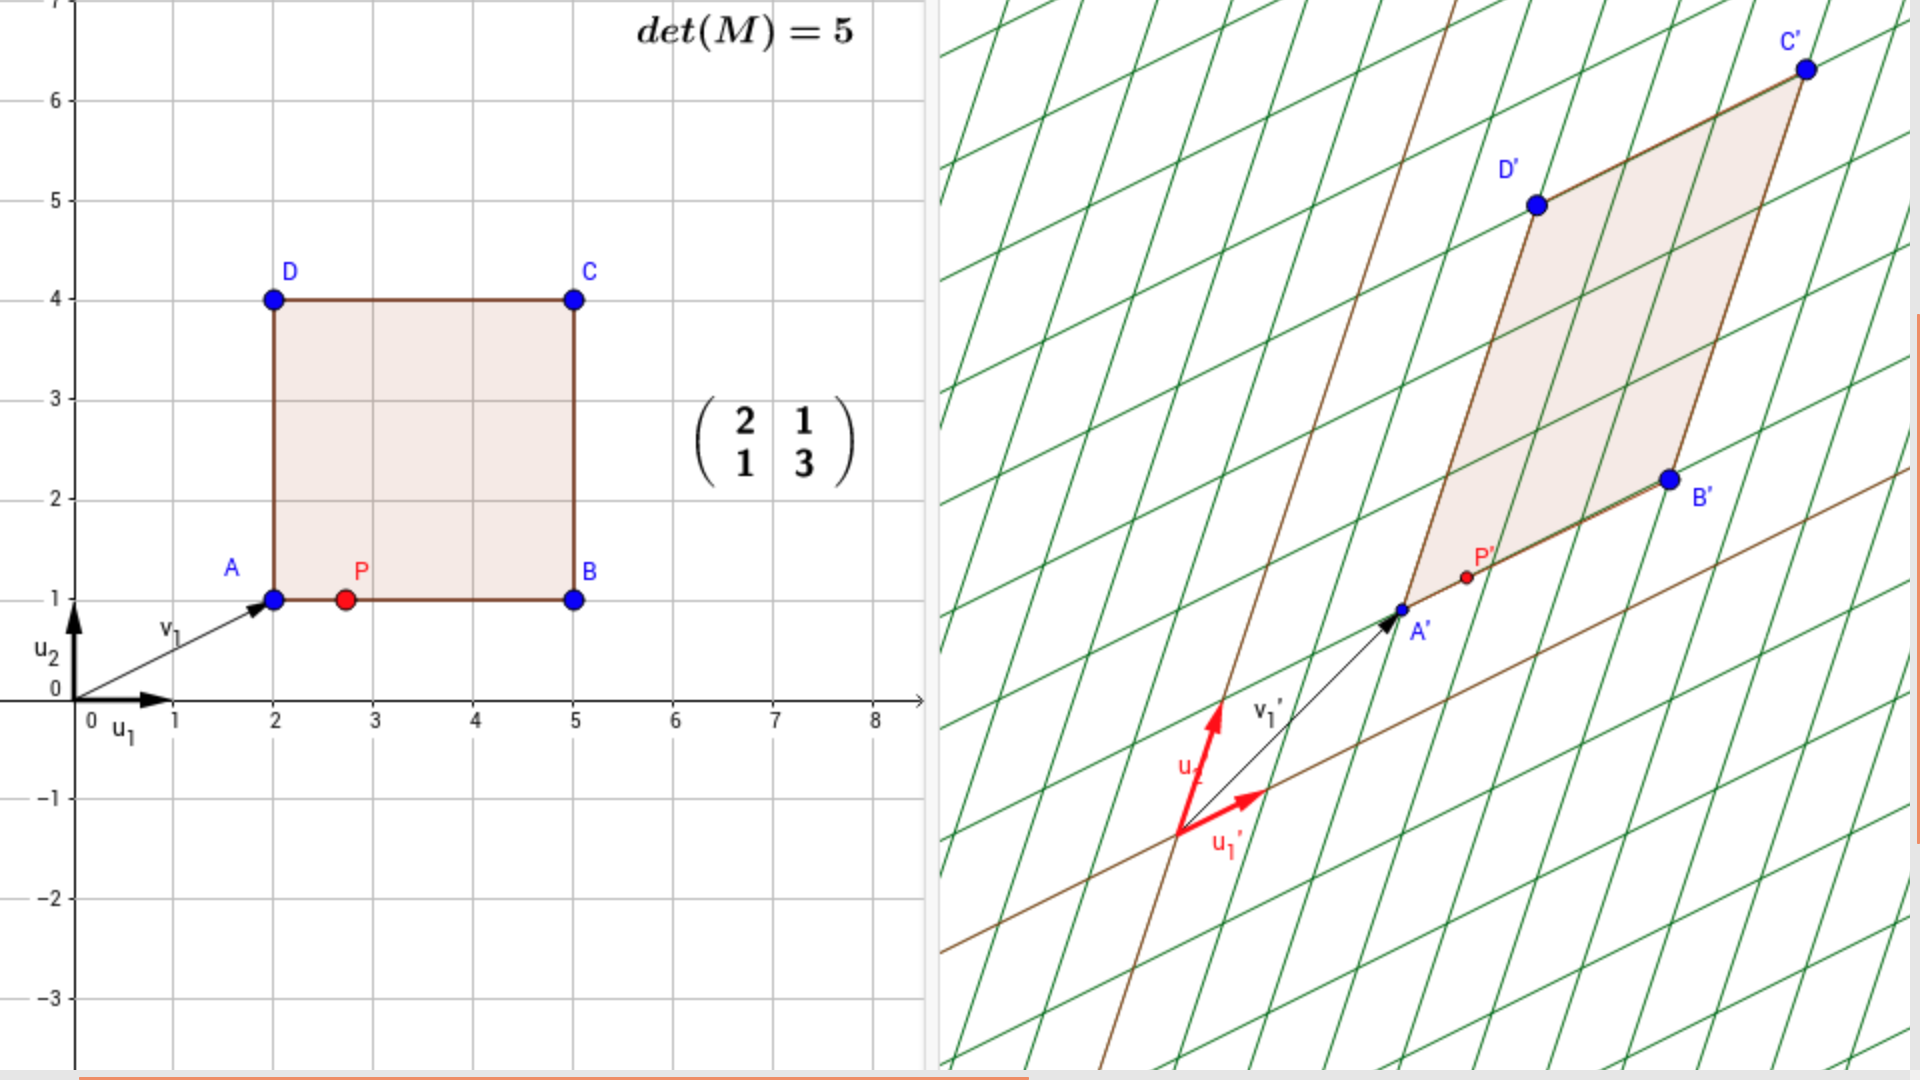
\includegraphics[scale=0.2]{matrix.png}
	\end{osservazione}
	\begin{osservazione}
		Se $u \parallel v$
	\end{osservazione}
\end{document}